
\documentclass[a4paper,UKenglish,cleveref, autoref, thm-restate]{lipics-v2021}
%This is a template for producing LIPIcs articles. 
%See lipics-v2021-authors-guidelines.pdf for further information.
%for A4 paper format use option "a4paper", for US-letter use option "letterpaper"
%for british hyphenation rules use option "UKenglish", for american hyphenation rules use option "USenglish"
%for section-numbered lemmas etc., use "numberwithinsect"
%for enabling cleveref support, use "cleveref"
%for enabling autoref support, use "autoref"
%for anonymousing the authors (e.g. for double-blind review), add "anonymous"
%for enabling thm-restate support, use "thm-restate"
%for enabling a two-column layout for the author/affilation part (only applicable for > 6 authors), use "authorcolumns"
%for producing a PDF according the PDF/A standard, add "pdfa"

% listing language definitions for several language of the following kinds:
% * ontology languages
% * markup languages
% * other semantic web languages
% * other languages occurring in the above contexts
% 
% for some related languages see also https://svn.kwarc.info/repos/stex/trunk/sty/etc/lstomdoc.sty
% 
% compiled by Christoph Lange (Universität Bremen, Jacobs University Bremen, University of Birmingham)
% 2010–2013
% math.semantic.web@gmail.com
% 
% https://github.com/clange/latex
% 
% For Mizar, see https://raw.github.com/JUrban/mizarmode/master/lstlangmizar.sty by Josef Urban

% Isabelle
% http://isabelle.in.tum.de
% partial specification; poor man's alternative to Isabelle's own LaTeX export
% but see also pmisabelle.sty
%\newif\iflst@instring\lst@instringfalse
%\newcommand*{\lst@eat}[1]{}%
%\newcommand*{\togglelst@instring}{%
%\upshape%
%\global\lst@instringfalse''
%}
\RequirePackage{xcolor}
\definecolor{IsabelleTypeColor}{HTML}{9f2ae5}
% Strings usually have this background color
% however listings has currently not support for selected background coloring
\definecolor{IsabelleStringBackground}{HTML}{535353}
\definecolor{IsabelleKeywordColor}{HTML}{2f769e}
\lstdefinelanguage{Isabelle}[]{ML}%
{morekeywords={%
abbreviation,% added by NM
assume,%
assumes,%
by,%
def,%
datatype,% added by NM
definition,% added by NM
fix,%
fixes,%
from,%
have,%
lemma,%
obtain,%
proof,%
partial\_function,%
qed,%
return,%
show,%
shows,%
theorem,%
typedef,%
try,%
unfolding,%
using,%
where,%
},
% modyfied to display highlighting inside strings
morestring=**[d][\color{IsabelleStringBackground}]{"},
% and highlight type prefixes (')
%moredelim=[s][\color{IsabelleTypeColor}]{'}{\ },
%added by NM
%moredelim=[s][\color{IsabelleStringBackground}]{(*}{*)},
basicstyle=\itshape,%
keywordstyle=\upshape\bfseries,%\color{IsabelleKeywordColor},%
columns=fullflexible,%
showstringspaces=false,%
mathescape,%
}[keywords,comments]


%\pdfoutput=1 %uncomment to ensure pdflatex processing (mandatatory e.g. to submit to arXiv)
%\hideLIPIcs  %uncomment to remove references to LIPIcs series (logo, DOI, ...), e.g. when preparing a pre-final version to be uploaded to arXiv or another public repository

\graphicspath{{./figures/}}%helpful if your graphic files are in another directory

\bibliographystyle{plainurl}% the mandatory bibstyle

\title{A Verified Implementation of B$^+$-Trees in Isabelle/HOL}

%\titlerunning{Dummy short title} %TODO optional, please use if title is longer than one line

\author{Niels Mündler}{Department of Computer Science, ETH Zurich, Switzerland}{n.muendler@tum.de}{https://orcid.org/0000-0003-3851-2557}{}%TODO mandatory, please use full name; only 1 author per \author macro; first two parameters are mandatory, other parameters can be empty. Please provide at least the name of the affiliation and the country. The full address is optional. Use additional curly braces to indicate the correct name splitting when the last name consists of multiple name parts.

\author{Tobias Nipkow}{Department of Informatics, Technical University of Munich, Germany}{nipkow@in.tum.de}{https://orcid.org/0000-0003-0730-515X}{}

%\author{Peter Lammich}{Department of Computer Science, The University of Manchester, Great-Britain}{lammich@in.tum.de}{https://orcid.org/0000-0003-3576-0504}{}

\authorrunning{N. Mündler and T. Nipkow} %TODO mandatory. First: Use abbreviated first/middle names. Second (only in severe cases): Use first author plus 'et al.'

\Copyright{Niels Mündler} %TODO mandatory, please use full first names. LIPIcs license is "CC-BY";  http://creativecommons.org/licenses/by/3.0/

\begin{CCSXML}
    <ccs2012>
       <concept>
           <concept_id>10003752.10003790.10011742</concept_id>
           <concept_desc>Theory of computation~Separation logic</concept_desc>
           <concept_significance>500</concept_significance>
           </concept>
     </ccs2012>
\end{CCSXML}
    
\ccsdesc[500]{Theory of computation~Separation logic}
%TODO mandatory: Please choose ACM 2012 classifications from https://dl.acm.org/ccs/ccs_flat.cfm 

\keywords{Separation Logic, Verification, Refinement} %TODO mandatory; please add comma-separated list of keywords

\category{} %optional, e.g. invited paper

\relatedversion{} %optional, e.g. full version hosted on arXiv, HAL, or other respository/website
%\relatedversiondetails[linktext={opt. text shown instead of the URL}, cite=DBLP:books/mk/GrayR93]{Classification (e.g. Full Version, Extended Version, Previous Version}{URL to related version} %linktext and cite are optional

%\supplement{}%optional, e.g. related research data, source code, ... hosted on a repository like zenodo, figshare, GitHub, ...
%\supplementdetails[linktext={opt. text shown instead of the URL}, cite=DBLP:books/mk/GrayR93, subcategory={Description, Subcategory}, swhid={Software Heritage Identifier}]{General Classification (e.g. Software, Dataset, Model, ...)}{URL to related version} %linktext, cite, and subcategory are optional

%\funding{(Optional) general funding statement \dots}%optional, to capture a funding statement, which applies to all authors. Please enter author specific funding statements as fifth argument of the \author macro.

\acknowledgements{I want to thank Prof. Dr. Tobias Nipkow and Dr. Peter Lammich for their input and support when writing this thesis.}%optional

%\nolinenumbers %uncomment to disable line numbering



%Editor-only macros:: begin (do not touch as author)%%%%%%%%%%%%%%%%%%%%%%%%%%%%%%%%%%
\EventEditors{John Q. Open and Joan R. Access}
\EventNoEds{2}
\EventLongTitle{42nd Conference on Very Important Topics (CVIT 2016)}
\EventShortTitle{CVIT 2016}
\EventAcronym{CVIT}
\EventYear{2016}
\EventDate{December 24--27, 2016}
\EventLocation{Little Whinging, United Kingdom}
\EventLogo{}
\SeriesVolume{42}
\ArticleNo{23}
%%%%%%%%%%%%%%%%%%%%%%%%%%%%%%%%%%%%%%%%%%%%%%%%%%%%%%

\newcommand{\btree}{B$^+$-Tree}
\newcommand{\btrees}{B$^+$-Trees}

\begin{document}

\maketitle

%TODO mandatory: add short abstract of the document
\begin{abstract}
    In this thesis, we use the interactive theorem prover Isabelle/HOL \cite{DBLP:books/sp/NipkowPW02} to verify
    an imperative implementation of the ubiquitous \btree data structure \cite{DBLP:journals/acta/BayerM72}.
    The implementation supports point, insertion and range queries with efficient binary
    search for intra-node navigation. This is accomplished by first specifying the structure
    abstractly in the functional modeling language HOL and proving functional correctness.
    Using manual refinement, we derive an imperative implementation in Imperative/HOL
    \cite{DBLP:conf/tphol/BulwahnKHEM08}. We show the validity of this refinement using the separation logic utilities
    from the Isabelle Refinement Framework \cite{DBLP:conf/itp/Lammich19}. The code can be exported to the
    programming languages SML and Scala. Considering development time and lines of code, our approach
    compares well to other approaches at mechanized verifications of the \btree\ data
    structure, while being unique in supporting range queries and binary node internal search.
\end{abstract}

\section{Introduction}
\label{sec:introduction}


An important topic in computer science is the study of the
\textit{functional correctness} of an algorithm.
It states whether an algorithm satisfies specified
input/output behavior.
Proving correctness of an algorithm
becomes especially interesting when it is be applied
to directly executable code and even more so if it is machine checked.
Unfortunately, with both, the task becomes
significantly more complex.
Even in an abstract specification, where topics such as
memory management may be abstracted away,
machine checked proofs of non-trivial properties
are hard.
Furthermore for concrete implementations,
low-level decisions about memory allocation or
the eligibility of reusing variables need to be
reasoned about.
We provide a computer assisted proof in the interactive
theorem prover Isabelle/HOL \cite{DBLP:books/sp/NipkowPW02} for the functional
correctness of an imperative implementation of the \btree data-structure
and present how we dealt with the above mentioned issues.


In \autoref{sec:introduction}, we have a brief overview on related
work and introduce the definition of \btree used in our approach.
In order to verify an imperative version of the structure,
we define a functional, abstract specification of a tree operations
and prove functional correctness, by showing that structural invariants are preserved
and the obtained results are correct.
In a second step, we provide an imperative refinement
of the functional operation.
The correctness of the imperative version is shown by proving that it refines the functional specification.
Thus the proof obligation for the imperative implementation
is reduced to a proof of equivalence between the output of the
functional and the imperative implementation.
This process is repeated for each operation throughout
\autoref{sec:set} and \autoref{sec:imperative_iter}

Finally, we present learned lessons, compare the results with related work and suggest potential future
research in \autoref{sec:conclusion}.


\subsection{Motivation}
\label{sec:motivation}

\btrees form the basis of virtually all modern RDBMs.
Especially when employed in financial applications
or in safety critical software it is vital that
no data is lost or corrupted.
Meanwhile, even single-threaded databases
are non-trivial to analyse and verify,
especially machine-checked.
The only work in the literature on that topic
is the work by Malecha %todo cite
However, it lacks a number of common features for \btree
interaction, such as range searches and efficient binary search.
Moreover, it is bound to the Coq interactive theorem prover.
With this work, we intend to enrich the canon on verified
\btrees with an efficient and modular implementation
in Isabelle/HOL.


\subsection{Related Work}
\label{sec:related_work}

There exist two pen and paper proofs via the rigorous approach
by Fielding \cite{Fielding80} and Sexton \cite{DBLP:journals/entcs/SextonT08}.
They pioneered in suggesting tools for analysing \btrees,
showing how refinement and separation logic can be used to
derive convincing proofs easily.

Among imperative implementations, two machine checked proofs exist as well.
In the work of Ernst \cite{DBLP:journals/sosym/ErnstSR15},
an imperative implementation is directly verified
by combining interactive theorem proving
with shape analysis.
The main recursive procedures are interactively verified in KIV.
Data structure properties such as circle-freeness are then proven by shape-analysis.
Another direct proof on an imperative implementation
was conducted by Malecha \cite{DBLP:conf/popl/MalechaMSW10}, with the YNOT
extension to the interactive theorem prover Coq.
Both works use recursively defined "shape predicates"
that describe formally how the nodes and pointers
represent an abstract tree of finite height.
Similar to the work of Malecha, we define these predicates functionally
and derive finiteness and acyclicity from the relation between imperative and functional specification.

\section{Contributions}

In this work, we derive our own definition of B-trees
by combining the original definition
with approaches that have resulted in verified implementations previously.
Based on the definition, we specify the B-tree data structure in the
functional modeling language HOL.
The specification is complemented by a proof of its correctness
with respect to refining a set of linearly ordered elements.
All proofs are machine-checked in the Isabelle/HOL framework,
an interactive automated theorem prover \cite{DBLP:books/sp/NipkowK14}.
Within the framework,
the functional specification already yields automatic extraction of executable,
but inefficient code.

Using manual refinement, we derive an imperative implementation of the functional specification
in Imperative/HOL.
For this purpose, we introduce static arrays with variable size
and efficient copy and move operations on arrays.
The implementation is defined with respect to some abstract imperative
operation for node-internal navigation.
We provide one such operation that employs linear search,
and one that conducts binary search.
All imperative programs are shown to refine the functional specifications
using the separation logic utilities from the Isabelle Refinement Framework by
Lammich \cite{DBLP:journals/jar/Lammich19}.

This process results in a proof of the functional correctness
of an imperative implementation of the B-tree data structure.
The implementation supports set membership and insertion queries
and uses efficient binary search for intra-node navigation.
As with every specification in Imperative/HOL,
automatic executable code extraction to
several functional programming languages is supported.
In addition, we provide a proof of the logarithmic relationship between height and number of nodes,
reproducing results of Bayer \cite{DBLP:journals/acta/BayerM72}.
This verifies claims on the efficiency of
operations on the tree.


Ernst verified a simplified version of \btrees that does
not have links between leaf nodes.

Malecha already built and verified \btrees \cite{}.
In their approach, they chose an intermediate layer of a functional
data structure that explicitely stores pointers to their heap embedded
correspondence.

\subsection{Contributions}
\label{sec:contributions}

We provide an alternative approach to verifying \btree implementations,
by separating the functional specification and the imperative implementation.
This allows for complex relationships to be validated on a purely
functional level, while on the imperative level
only refinement of the abstract operations needs to be shown.
The approach allowed us to supplement the implementation
with an efficient binary search on the node level
and eventually provide an efficient range query iterator
on top of a list element iterator.


\section{\btrees\ and Approach}
\label{sec:approach}

The \btree is a ubiquitous data structure to efficiently retrieve and manipulate
indexed data stored on storage devices with slow memory access \cite{DBLP:journals/csur/Comer79}.
They are $n$-ary balanced search trees, where $n$ is a free parameter.
We specify them as implementing a set interface,
where all elements in the leaves are comprising the content of an abstract set.
The inner nodes only contain separators to guide the recursive navigation through the tree.

Further the leaves usually contain pointers
to the next leaf, allowing for efficient iterators and range queries.

The goal of this work is to define this data structure
and implement and verify efficient heap-based imperative operations on them.
For this purpose, we introduce a functional, algebraic definition and
specify all invariants on this level.
It is important to note that this representation is not complete,
as we can not express the aliased pointers to the next leaf in a meaningful
way on the algebraic level.
However important structural invariants, such as sortedness and balancedness
can be verified.

In a second step an imperative definition is introduced,
that takes care of the refinement of linked lists to arrays in the heap
and introduces (potentially shared) pointers instead of algebraic structures.
Using a refinement relationship, we can prove that an imperative refinement
of the functional specification preserves the structural invariants
of the imperative tree on the heap.
The only remaining proof obligation on this level is to ensure the correctness
of the leaf pointers.


\subsection{Definitions}
\label{sec:data_structure_defs}

% TODO shorten

The algebraic \btree is defined as follows:

\begin{lstlisting}[mathescape=true, language=Isabelle,label=lst:btree-def]
datatype 'a bplustree =
    LNode ('a list) |
    Node (('a bplustree * 'a ) list) ('a bplustree)
\end{lstlisting}


\begin{figure}
    \centering
    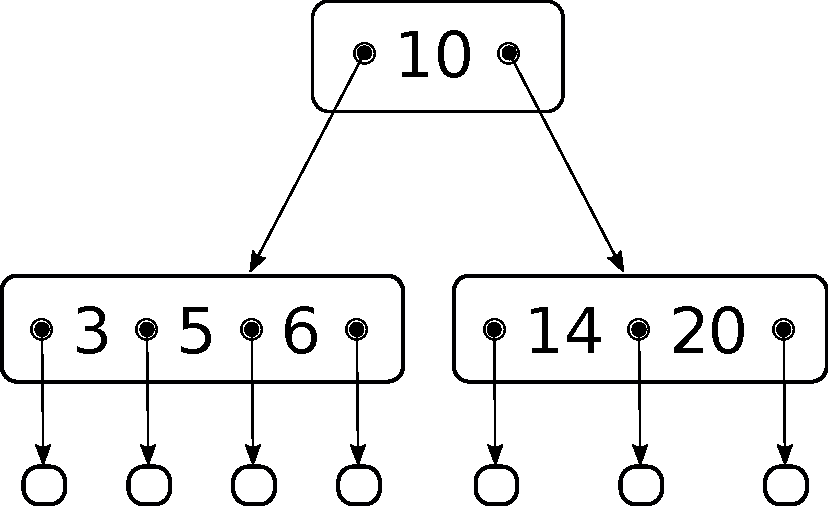
\includegraphics[width=0.5\linewidth]{btree-basic-nopair.pdf}
    \caption[Visualization of a \btree]
    {Nodes contain several elements, the internal list/array structure is not depicted.
    The dotted lines represent links to following leaf nodes that are not present in the algebraic formulation.}
    \label{fig:btree-basic}
\end{figure}


Every node contains a list of \textit{keys} (also \textit{separators}, and \textit{subtrees} (\textit{children}),
that represent further \btree nodes.
The separators and subtrees may be considered interleaved within a node,
such that we can speak of a subtree to the left of a separator and
a subtree to the right of a separator,
where for a separator at index $i$ we mean the subtree in the respective
subtree list at index $i$ and $i+1$ respectively.
Note that this already implies that the list of subtrees is one
longer than the list of separators - we refer to the last subtree
as the \textit{last} or \textit{dangling} subtree.
The leafs contain a list of \textit{values}.
A \btree with above structure must fulfill the properties
\textit{balancedness}, \textit{order} and \textit{alignment}.

\textbf{Balancedness} requires
that each path from the root to any leaf has the same length $h$.
In other words, the height of all trees in one level of the tree must be equal,
where the height is the maximum path length to any leaf.

In general terms, the property of \textbf{order} ensures a certain minimum and maximum
number of subtrees for each node.
A \btree is of order $k$, if each internal node has at least $k+1$
subtrees and at most $2k+1$.
The root is required to have a minimum of 2 and a maximum of $2k+1$ subtrees.
We require that $k$ be strictly positive, as for $k = 0$ the requirements on the tree
root are be contradictive.
%TODO insert more detailed reason?

Further the keys and values must be sorted within the tree.
We define this by two separate properties: \textbf{Alignment}, which means that all keys stored
in the subtree to the left of a separator are smaller than the value of the separator
and all indices in the subtree to the right are greater or equal.
\footnote{
    The exact direction of the part that may contain equal element is a design choice.
}
\begin{lstlisting}[mathescape=true, language=Isabelle,label=lst:btree-alignment-def]
fun inbetween where
  inbetween f l Nil t u = f l t u |
  inbetween f l ((sub,sep)#xs) t u = (f l sub sep $\wedge$ inbetween f sep xs t u)

fun aligned :: "'a ::linorder $\Rightarrow$ _" where
  aligned l (LNode ks) u = (l < u $\wedge$ ($\forall$x $\in$ set ks. l < x $\wedge$ x $\le$ u)) |
  aligned l (Node ts t) u = (inbetween aligned l ts t u)
\end{lstlisting}


Note that this property can not be reduced to the sortedness of an inorder traversal,
because whether or not an element is allowed to be equal to a separator or not
depends on the precise structure of the tree, not only on its position in the inorder traversal.
Moreover the separator to the right of its preceding separator must be smaller,
implying sortedness of all lists within nodes.
Equivalently, all key lists within the leafs should be \textbf{sorted}.
We show the even stronger fact that the concatenation of all leaf lists
% TODO why actually?
is sorted in order to have a handy statement when reasoning about iterators.

The definition in \autoref{lst:btree-def} described an algebraic data structure.
It is by construction finite which lets us proof termination for recursive functions almost for free.
However, this structure also forbids sharing of pointers or local updates.
The goal of this paper is to derive an efficient implementation
of \btrees, which is why we define an imperative node that allows such operations.
Each imperative node contains pointers rather than the full subtree and
stores all values in arrays rather than linked lists.

\begin{lstlisting}[mathescape=true, language=Isabelle,label=lst:btree-imp-def]
datatype 'a btnode =
  Btnode (('a btnode ref option * 'a )) pfarray ('a btnode ref) |
  Btleaf ('a pfarray) ('a btnode ref option)
\end{lstlisting}

All elements of this tree can and will be stored on a heap, where \textbf{ref} is a pointer
to another element in the heap, \textbf{ref option} being a pointer that is potentially null.
With this setup, it is possible to modify elements on the heap or share pointers.
However, it is troublesome to conduct direct proofs on this structure.
We therefore introduce a refinement relation to the algebraic data structure.
In later steps we can then show that certain operations on the imperative
tree refine abstract functions and can thus imply relevant information on the obtained result and modified tree.

The relation is expressed as a separation logic formula that links an abstract tree to an
imperative data structure.
It takes an algebraic tree (\textbf{bplustree}) and an imperative tree
(\textbf{btnode ref}) as well as a first and last leaf.
In general, the relation states that all parts of the abstract tree
are refined by the content of the heap that represents the imperative tree.
The abstract linked list is itself refined by an array,
and the pointers on subtrees refine again the subtrees of the algebraic tree.

\begin{lstlisting}[mathescape=true, language=Isabelle,label=lst:btree-relation]
fun bplustree_assn where
  bplustree_assn k (LNode xs) a r z =
 ($\exists_A$ xsi fwd.
      a $\mapsto_r$ Btleaf xsi fwd
    * is_pfa (2*k) xs xsi
    * $\uparrow$(fwd = z)
    * $\uparrow$(r = Some a)
  ) |
  bplustree_assn k (Node ts t) a r z =
 ($\exists_A$ tsi ti tsi' tsi'' rs.
      a $\mapsto_r$ Btnode tsi ti
    * is_pfa (2*k) tsi' tsi
    * $\uparrow$(length tsi' = length rs)
    * $\uparrow$(tsi'' = zip (zip (map fst tsi') (zip (butlast (r#rs)) rs))) (map snd tsi'))
    * list_assn (($\lambda$ t (ti,r',z'). bplustree_assn k t (the ti) r' z') $\times_a$ id_assn) ts tsi''
    * bplustree_assn k t ti (last (r#rs)) z)
    )
\end{lstlisting}

The first and last leaf are part of the refinement relation because
we also need to express the fact that the leafs are correctly linked.
There is no abstract equivalent for the next pointers in the leafs.
For this reason, each subtree is passed the first leaf of its right neighbor
in order to ensure that this is the next pointer stored in the last leaf node.
Now how are these leaf pointers obtained on the higher levels?
The trick is that they are not obtained at all.
We just assume that there exists a list of such leaf pointers using an existential quantifier.
In order to ensure that this list is the correct one, we pass the supposedly
first leafs into each subtree.
It is passed on recursively to the leaf node,
where it is compared to the concrete pointer of that node.
This way, we can derive on the higher levels of the tree
that the obtained leaf pointer is in fact the correct one and pass it to the
neighboring subtree.

Even though the linking among the nodes is not used until we obtain
an iterator, we need to make sure that this property is maintained
during initialization and construction of the tree.
Therefore the pointers are an integral part of the refinement relation
and we need to proof that it is not violated when querying or inserting elements.

\subsection{Node internal navigation}
\label{sec:split}

In order to define meaningful operations that navigate
the node structure of the \btree,
we need to find a method that handles search within a node.
On binary trees, this question is simle, in each node we either choose
the left or right subtree.
For 2-3-4 trees as described by Nipkow \cite{DBLP:conf/itp/Nipkow16} the process becomes more tricky
but eventually a binary search like node internal traversal can be verified.
For general k-ary \btrees there have not been sophisticated search strategies.
Ernst \cite{DBLP:journals/sosym/ErnstSR15} and Malecha \cite{DBLP:conf/popl/MalechaMSW10}
both simply use a linear search through the node lists.
However, \btrees are supposed to have memory page sized nodes \cite{DBLP:journals/csur/Comer79}, 
which makes a linear search unfeasible in practical contexts.

Instead we propose a different approach.
In general we introduce a locale, a context in which we assume that we
have access to a function that correctly navigates through the node internal structure.
We call this function a $split$ function, and define it by some required behavior.
In general, given a list of separator-subtree pairs, the function should
return the pair containing the subtree that, according to the structural invariant of the \btree,
must contain the element that is being searched for or will hold the element after correct insertion.
A similar function is defined on the key lists of the leaf nodes.

Using this abstraction, all operations can be defined and verified
in the following sections.
In order to prove the context valid, we simply provide a linear search function
that provides exactly the required functionality.

Finally, when approaching imperative code extraction,
we show that a binary search based function refines the
functionality as well.
This binary search is directly implemented and verified on the imperative
level and is eventually plugged into the abstractly defined
imperative operations on the \btree.
Thus we obtain imperative code that makes use of an efficient
binary search, without adding complexity to the proofs.
The definition and implementation closely follows
the approach described in detail in the
verification of B-Trees \cite{DBLP:journals/afp/Mundler21}.


\section{Set operations}
\label{sec:set}

The most important operations on \btrees are point querys and insertion.
There is a canon on their implementation which we followed in our approach.

\subsection{Functional Point Query}
\label{sec:functional_pq}

The point query operation is straightforward.
For an inner node, find the correct subtree which must contain
the searched value, if it is in the tree.
Then recursively search for the value in that subtree.
Inside the leaf node, search directly in the list of values.

\begin{lstlisting}[mathescape=true, language=Isabelle,label=lst:isin-def]
fun isin:: "'a bplustree $\Rightarrow$ 'a $\Rightarrow$ bool" where
  isin (LNode ks) x = (isin_list x ks) |
  isin (Node ts t) x = (case split ts x of
     (_,(sub,sep)#rs) $\Rightarrow$ isin sub x
   | (_,[]) $\Rightarrow$ isin t x
  )
\end{lstlisting}

Note that we assume here that a "split" and "isin\_list" operation exist,
as described in \autoref{sec:split}.
Since this function does not modify the tree involved at all,
we only need to show that it returns the correct value.


\begin{lstlisting}[mathescape=true, language=Isabelle,label=lst:isin-set-inorder]
theorem isin_set_inorder:
  assumes "sorted_less (leaves t)"
    and "aligned l t u"
  shows "isin t x = (x $\in$ set (leaves t))"
\end{lstlisting}

In general these proofs on the abstract level are made
based on another refinement relation suggested by Nipkow. \cite{DBLP:conf/itp/Nipkow16}
In this relation, we say that the \btree refines a sorted list of its leaf elements.
This way, we argue that recursing into a specific subtree
is equivalent to splitting the list of leaves at the correct position
and searching in the correct sublist.
The same approach was applicable for proving the correctnes of functional
operations on B-Trees. \cite{DBLP:journals/afp/Mundler21}

The proofs on the functional level therefore turn out to be very succinct.
With the correctness of this operation,
we go on and define an imperative version of the operation that
refines each step of the abstract tree to an operation on the imperative tree.

\subsection{Imperative Point Query}
\label{sec:imperative_pq}

The imperative version of the point query is a partial function.
This means that termination is not guaranteed anymore,
at least without further assumptions.
This is inevitable since one could pass cyclic trees into the function.
However, we will later show that, if the input refines an abstract tree,
the function terminates and is correct.

\begin{lstlisting}[mathescape=true, language=Isabelle,label=lst:isin-imp-def]
partial_function (heap) isin :: "'a btnode ref $\Rightarrow$ 'a $\Rightarrow$  bool Heap"
  where
    "isin p x = do {
  node \<leftarrow> !p;
  (case node of
     Btleaf xs _ $\Rightarrow$ imp_isin_list x xs |
     Btnode ts t $\Rightarrow$ do {
       i \<leftarrow> imp_split ts x;
       tsl \<leftarrow> pfa_length ts;
       if i < tsl then do {
         s \<leftarrow> pfa_get ts i;
         let (sub,sep) = s in
           isin (the sub) x
       } else
           isin t x
    }
)}"
\end{lstlisting}

Again, we assume that there are split functions that do node internal search operations for us
and themselves refine their functional equivalent.
Note how the imperative function does not actually split
the internal array, but rather returns the index of the element
that would have been returned by the abstract split function.
Therefore the pattern matching against a returned pair
is replaced by comparing the index to the length of the list.

In order to show that the function returns the correct result,
we merely show that it does the same operation on the imperative tree
as on the algebraic tree.
This proof can be done inductively on the structure of the abstract tree.

\begin{lstlisting}[mathescape=true, language=Isabelle,label=lst:isin-refines]
lemma  
   assumes "k > 0" and "root_order k t"
    and "sorted_less (inorder t)" and "sorted_less (leaves t)"
   shows
   "<bplustree_assn k t ti r z>
     isin ti x
   <$\lambda$y. bplustree_assn k t ti r z * $\uparrow$(abs_split_set.isin t x = y)>$_t$"
\end{lstlisting}

Assuming structural soundness of the abstract tree that is refined by the pointer passed to the function,
we obtain that the returned result is equivalent to the result returned by the abstracted function.
Further we must explicitely show that the tree on the heap
still refines the same abstract tree after the operation,
which was implicit on the abstract level.

The insertion operation and its proof largely line up with the approach to point queries.
But since insertion modifies the tree,
we need to additionally show on the abstract level that the modified tree
maintains the invariants required for the \btree.
By showing that the obtained tree after the imperative insert operation
refines the modified abstract tree, it follows that the imperative tree
also maintains these invariants.

Moreover, we need to show that the leaf pointers
maintain correct linking after the operation.
This can only be shown on the imperative level as there is no abstract equivalent
to the shared pointers.
As the correct linking of leaf pointers is part of the refinement relation,
this proof obligation is part of the proof of refinement of the abstract insertion.


% TODO details on the choice of implementation for the operation?

%\subsection{Functional Insert}
%\label{sec:functional_insert}
%
%The definition of insertion is largely lined up with the definition
%of point queries.
%
%\subsection{Imperative Insert}
%\label{sec:imperative_insert}
%
%One additional challenge here is to prove the correct initialization
%and modification of pointers in the leaves,
%as this cannot be proven on the abstract level, where these pointers
%have no correspondence.

Deletion is less commonly implemented and even less verified,
however we provide a verified functional definition of deletion and a definition of an imperative refinement.
Showing the correctness of the imperative version would largely follow
the same pattern as the proof of the correctness of insertion.



\section{Range operations}
\label{sec:range}

On the functional level, the forwarding leaf pointers in each leaf
are not present, as this would require aliasing.
Therefore, the abstract equivalent of an iterator
is simply a concatenation of all leaf contents by
trivially copying them together recursively.
%Range iterators then concatenate the correct parts of the abstract tree.
When refining the operations, we will make use of the leaf pointers
to obtain an efficient implementation.

\subsection{Iterators}
\label{sec:imperative_iter}

From an implementation perspective, obtaining an iterator over the leafs
of a \btree is trivial.
We simply recurse down the tree to obtain the first leaf and from there follow leaf
pointers along the skirt of the tree until we reach the final leaf marked by a null next pointer.
However, from a refinement relation perspective the situation is a bit more intricate.
It is important to find a recursive formulation of the linked list in the leaf pointers.
At the same time, we want to maintain enough information about the remainder of the tree
to be able to reconstruct the assertion about the whole tree.
However, we can not simply express the linked list view and the view on the
whole tree at the same time,
as separation logic forces us not to make statements about the contents of
any memory location twice.
This is an important feature of separation logic,
in order to keep the parts of the heap disjunct and
thus be able to independently modify parts of the heap assertion.

We therefore follow the approach of \cite{DBLP:conf/popl/MalechaMSW10} and
try to find an equivalent formulation that separates the whole tree in a
view on its inner nodes and the linked leaf node list.
The main idea to keep the heaps separate is to
assert correct content of the leafs within the linked list part
and only assert that the pointers on leafs in the inner nodes part
are equal to the leaf pointers in the linked list, but not accessing
their content at all (which would be a second memory access).

A first attempt to use \autoref{lst:btree-relation} for this fails.
The reason is, that we can not express that the linked leaf nodes
are precisely the leaf nodes that the lowest level of inner nodes point to.
We can show that the whole tree can be separated into a linked list in the leafs
and some remainder of the heap, but we can not show that we can necessarily transform
these two statements back together and obtain a structurally consistent \btree.

\begin{lstlisting}[mathescape=true, language=Isabelle,label=lst:btree-view-split-oneway]
lemma bplustree_leaf_nodes:
  "bplustree_assn k t ti r z $\Longrightarrow_A$ leaf_nodes_assn k (leaf_nodes t) r z * true"
\end{lstlisting}

% TODO graphic explaining the issue
\begin{figure}
    \centering
    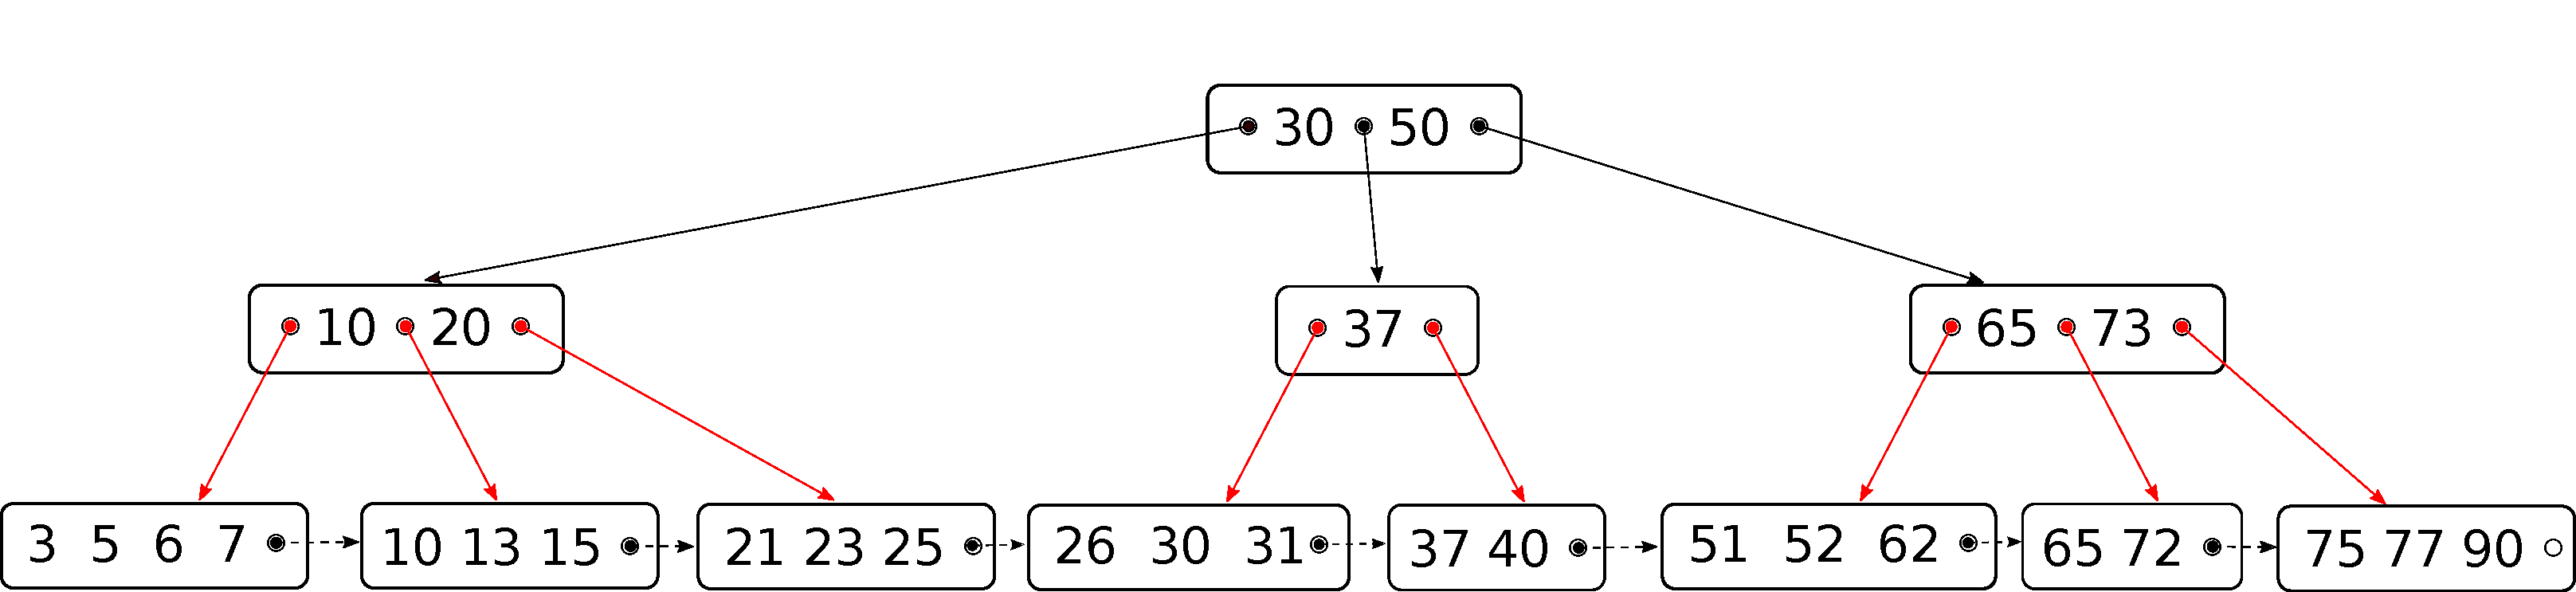
\includegraphics[width=1\linewidth]{btree-view-split.pdf}
    \caption[Split view of the \btree]
    {In order to obtain separate assertions about the concatenated leaf list
    and the internal nodes of the tree, the structure is abstractly split along the
    pointers marked in red. In order to be able to combine the views together later,
    the marked pointers have to be extracted to show explicitly that they are shared.}
    \label{fig:btree-view-split}
\end{figure}

In a second attempt we succeed by making the sharing explicit.
We extract from the whole tree the precise list of pointers to leaf nodes
in the correct order as visualized in \autoref{lst:btree-view-split}.
We express this new view by extending the existential quantifier in \autoref{lst:btree-lst:btree-relation}
to assume that there is a partition of all leaf pointers,
such that each subtree has exactly its part of the partition as leaf pointers.
In the separated view, we now require that the pointers
in the lowest level of the inner node view are precisely the pointers
that are comprising the linked list view of the leafs.
A convenient fact is that the view on the tree that makes the leaf pointers explict
is equivalent to the view where we do not know precisely which pointers are in the leafs.
The statement from \autoref{lst:btree-relation} is strong enough to guarantee that such a list exists.


\begin{lstlisting}[mathescape=true, language=Isabelle,label=lst:btree-view-split]
fun bplustree_assn_leafs where
    bplustree_assn_leafs k (LNode xs) a r z leafptrs =
   ($\exists_A$ xsi fwd.
        a $\mapsto_r$ Btleaf xsi fwd
      * is_pfa (2*k) xs xsi
      * $\uparrow$(fwd = z)
      * $\uparrow$(r = Some a)
      * $\uparrow$(leafptrs = [a])
    ) |
    bplustree_assn_leafs k (Node ts t) a r z leafptrs =
   ($\exists_A$ tsi ti tsi' tsi'' rs split.
        a $\mapsto_r$ Btnode tsi ti
      * bplustree_assn_leafs k t ti (last (r#rs)) (last (rs@[z])) (last split)
      * is_pfa (2*k) tsi' tsi
      * $\uparrow$(concat split = leafptrs)
      * $\uparrow$(length tsi' = length rs)
      * $\uparrow$(length split = length rs + 1)
      * $\uparrow$(
          tsi'' = zip (zip (map fst tsi') (zip (butlast (r#rs))
          (zip rs (butlast split)))) (map snd tsi')
        )
      * list_assn (
          ($\lambda$ t (ti,r',z',lptrs). bplustree_assn_leafs k t (the ti) r' z' lptrs)
           $\times_a$ id_assn
        ) ts tsi''
      )


lemma bplustree_extract_leafs:
    "bplustree_assn k t ti r z = ($\exists_A$leafptrs. bplustree_assn_leafs k t ti r z leafptrs)"

lemma bplustree_leaf_nodes_sep:
  "bplustree_assn_leafs k t ti r z lptrs =
   leaf_nodes_assn k (leaf_nodes t) r z lptrs * inner_nodes_assn k t ti r z lptrs"
\end{lstlisting}

In the work of Malecha \cite{DBLP:conf/popl/MalechaMSW10}, 
this list of precise leaf pointers is exactly the list of abstract leafs,
as the abstract leafs each contain the precise heap pointer they are refining.
Keeping the two layers separate leads to the need of specifying
exactly at which point the actual pointers are relevant
and where we are satisfied by knowing that a pointer refines
an abstract tree.

Now to obtain an iterator on the leaf nodes of the tree,
we simply obtain the first leaf by a recursive function, leaving
us with a tree refining an abstract tree and the pointer to its first leaf.

\begin{lstlisting}[mathescape=true, language=Isabelle,label=lst:btree-first-leaf]
lemma first_leaf_rule:
  assumes "k > 0" and "root_order k t"
  shows "<bplustree_assn k t ti r z>
  first_leaf ti
  <$\lambda$u. bplustree_assn k t ti r z * $\uparrow$(u = r)>$_t$"
\end{lstlisting}


On the result, we can apply the view split from \autoref{lst:btree-lst:btree-view-split}
to realize that we now have a pointer that provides a list-recursive
view on the leaf elements and the inner nodes on the remaining heap.
In a next step, we show that such a list view can be used
to define an imperative iterator over the refined list,
fulfilling the list iterator interface from Lammich. \cite{DBLP:conf/itp/Lammich19}

To really obtain an iterator that returns every single element of the
leaf nodes, rather than the leaf nodes or the contained arrays themselves,
we introduce a flattening iterator.
It takes an outer iterator over a data structure \textit{a} that returns elements of type \textit{b},
and inner iterator over the data structure \textit{b}.
The result is instantiated code that refines an iterator
over the concatenated list of elements refined by the outer iterator.

Using this structure, we obtain a function that creates an iterator
over the leafs of the original tree.
Note how all notion of the explicitely shared leaf pointers
has disappeared on this level, as their existence was hidden within the definition
of the leaf elements iterator.

\begin{lstlisting}[mathescape=true, language=Isabelle,label=lst:btree-view-split]
lemma leaf_elements_iter_init_rule:
  assumes "k > 0" and "root_order k t"
  shows "<bplustree_assn k t ti r None>
    leaf_elements_iter_init ti
    <$\lambda$it. leaf_elements_iter k t ti r (leaves t) it>$_t$"
\end{lstlisting}

\subsection{Range operations}
\label{sec:imperative_range}

A common use case of \btrees
is the obtaining of a lower bound on some key
or to obtain  all elements within a certain range. \cite{DBLP:journals/ftdb/Graefe11}
A lower bound and the beginning of a range iterator
can be both obtained in logarithmic time, making use of the tree structure.
The operation is similar to the point query operation,
only that it does not return whether or not the
found element is equal but an iterator starting at this element.
The range bounded from below is all elements returned by the iterator,
the first element being the lower bound.

\begin{lstlisting}[mathescape=true, language=Isabelle,label=lst:btree-lrange]
fun lrange:: "'a bplustree $\Rightarrow$ 'a $\Rightarrow$ 'a list" where
    "lrange (LNode ks) x = (lrange_list x ks)" |
    "lrange (Node ts t) x = (
        case split ts x of (_,(sub,sep)#rs) $\Rightarrow$ (
               lrange sub x @ leaves_list rs @ leaves t
        )
     | (_,[]) $\Rightarrow$ lrange t x
    )"
\end{lstlisting}
  
Again, we assume that there exists a function \textit{lrange} that
obtains the lower bounded range from a list of sorted elements.
Note how the abstract function explicitely recurses into
remaining parts of the tree and constructs lists on the leaves by concatenating them.
This will not be the case in the refined version anymore
as we know that the iterator comprises all elements in the remainder of the tree.

However showing this turns out to be not as straightforward
as expected, exactly due to this recursive step.
The reason is that iterators can only be expressed on a complete tree,
where the last leaf is explicitely a null pointer.\footnote{
    The issue is a technicality. Iterators have a \textit{has\_next} function
    that returns whether there are any remaining elements.
    In order to tell, we compare the leaf with the last leaf of the tree.
    If this is a valid leaf node (not a null pointer) we need to show
    that the linked leaf list is not cyclic - a proof obligation
    that can be omitted in the linked list view.
    % TODO more precise?
}
This contrasts the linked list view of the tree that can be expressed
recursively on subtrees.

Therefore we introduce an alternative formulation of the
abstract function, similar in thought to how we obtained the iterator
on the list from the first leaf of the tree.
In a first step, we obtain the correct list of leaf nodes
based on the binary search through the tree.
In a second step, we obtain the head of the list and apply
the function that returns the lower bounded range of elements within
and concatenate it with the other lists in the returned list of leaf nodes.
This way, the refinement of the tree internal search
can be conducted by only splitting the tree assertion into the linked-list view of the leafs
and the internal nodes.
Only when we have obtained the correct list for the whole tree,
where the last element is a null pointer,
we transform the result into the leaf element iterator.

\begin{lstlisting}[mathescape=true, language=Isabelle,label=lst:btree-leafs-range]
lemma concat_leafs_range_rule:
    assumes "k > 0" and "root_order k t" 
    and "sorted_less (leaves t)" and "Laligned t u"
    shows 
 "<bplustree_assn k t ti r None>
  concat_leafs_range ti x
  <leaf_elements_iter k t ti r (abs_split_range.lrange t x)>$_t$"
\end{lstlisting}

% TODO vis


\section{Conclusion}
\label{sec:conclusion}

\subsection{Lessons learnt}

It was interesting to notice that it is rather complicated
to even express, not to speak of attempting to prove acyclicity
 along the leaf nodes of the tree, as soon as the linked list was converted into an iterator.
Fortunately, we found a way around this issue, by only considering
the complete list of nodes whenever we turned them into
iterators. In that case, they were terminated by \textit{None}
which we could guarantee not to occur earlier in the list.

Moreover, handling statements on assertions has always been
a bit tedious throughout the project.
A major alleviation was the introduction of a specialized tool
that would substitute multiplicative terms in the formular
regardless of the disctribution in the original term.
This way, we could exchange equivalent assertions that comprised
multiple terms, like the combination of leaf view and trunk view,
with ease.
A future that is currently missing in the implementation of the entailment
proof tool, is that terms that could already be derived
would be removed in an intermediate proof state,
much like the simplifier removes terms in equation that could
already be shown to be equivalent and leaves only the remaining subterms.

\subsection{Evaluation}


The \btree implemented by Ernst features point queries and insertion,
however explicitely leaves out pointers within the leaves,
which forbids the implementation of iterators.
This work is also similar in nature to the part of the work of Malecha
that provides a \btree implementation.
In addition to the functionality provided in their work, we extend
the implementation with the missing Range iterator
and supply a binary search within nodes, as well as a modular approach
to further substitutionss.

With respect to the effort in lines of code and proof, we see
that our approach is similar to the effort by Malecha.
% TODO comparison LOC/LOP with Malecha, Ernst

\begin{figure}
    \centering
    \begin{tabular}{l|c|c|c}
        \                & \cite{DBLP:conf/popl/MalechaMSW10}$^{+}$ & \cite{DBLP:journals/sosym/ErnstSR15}$^{d}$ & Our approach$^{+}$ \\
        \hline
        Functional code &   360      & -                    & 324  \\ %TODO update
        Imperative code &   510      & 1862                  & 170  \\
        Proofs          &  5190      & 350 + 510 + 2940\footnotemark[7] & 2753 \\
        Timeframe (months) &  -     & 6+                      & 12   \\
    \end{tabular}
    \caption[Comparison of (unoptimized) Lines of Code and time investment in related mechanized \btree verifications.]
    {Comparison of (unoptimized) Lines of Code and time investment in related mechanized \btree verifications.
    The marker $^d$ denotes that the implementation verifies deletion operations, whereas $^+$ denotes the implementation of iterators.
    }
    \label{fig:proof-comparison}
\end{figure}
\footnotetext[7]{
    The proof integrates TVLA and KIV, and hence comprises
    explicitely added rules for TVLA (the first number),
    user-invented theorems in KIV (the second number)
    and "interactions" with KIV (the second number).
    Interactions are i.e. choices of an induction variable, quantifier instantiation
    or application of correct lemmas.
    We hence interpret them as each one apply-Style command and hence
    one line of proof.
}

\subsection{Future Work}

This work extends the canon on veryfied \btree
implementations.
Some additional features will be necessary for
usage in real-life scenarios.

A small addition to provide a true
range query can be provided by wrapping the lower-bounded
range iterator with an iterator
that stops iteration when the next element
would exceed the upper bound.

This work is still lacking a verified imperative version
of the deletion function.
We are expecting this proof to roughly follow
the approach used for point queries and insertion.

One important step towards efficient
\btree implementations that can be deployed
in realistic scenarios, is the migration of this code
to Isabelle-LLVM. \cite{DBLP:conf/itp/Lammich19}
At the beginning of this work, the code generator did
not yet support recursive data structures, but since
this functionality was added recently \btrees would be an interesting application.
Expectedly, the main difference will be the usage of Bitwords
instead of unbound natural numbers.

Finally, \btrees are supposed to write the contained
memory out to disk in order to maintain the durability constraint
usually required for databases.
This implementation lacks any interaction with IO systems.
We expect the formalization of correct interaction 
to be a particulary tricky task.

% TODO some analysis of the code generated? even necessary?

\bibliography{lipics-v2021-bplustrees}

\end{document}
